\chapter{Mesh Renumbering}\label{chapter:renumbering}

The \acrshort{acr:DG-SEM} solver described in this work is able to process unstructured meshes, to
be more general and perform computations on pre-constructed meshes. The program utilises the Hilbert
curve, a \acrlong{acr:SFC}, to preserve locality and reduce the size of inter-\acrshort{acr:GPU}
boundaries. The curve is described in Section~\ref{section:load_balancing:hilbert_curve}. These two
capabilities are at odds, as the overwhelming majority of meshes created for other purposes will not
be numbered according to the Hilbert curve. Also, the Hilbert curve is only defined for square
domains with \(n\) axis-aligned quadrilateral elements in the \(x\) and \(y\) directions, where
\(n\) is a power of two. Therefore, most off-the-shelf meshes will not inherit the good locality and
small boundaries between mesh blocks that we put a lot of effort to achieve in
Chapter~\ref{chapter:load_balancing}. Not only that, but there is even a performance penalty when
using a single \acrshort{acr:GPU} if elements that are close in the ordering are not geometrically
close, as memory access patterns are compromised. An extreme example is the original mesh used for
Section~\ref{section:results:complex_meshes}. Figure~\ref{fig:mesh_unsorted} shows the ordering of
the elements and how the mesh is split into mesh blocks if partitioned into \(16\) blocks as-is. 

\begin{figure}[H]
	\centering
	\subfloat[Ordering]
	{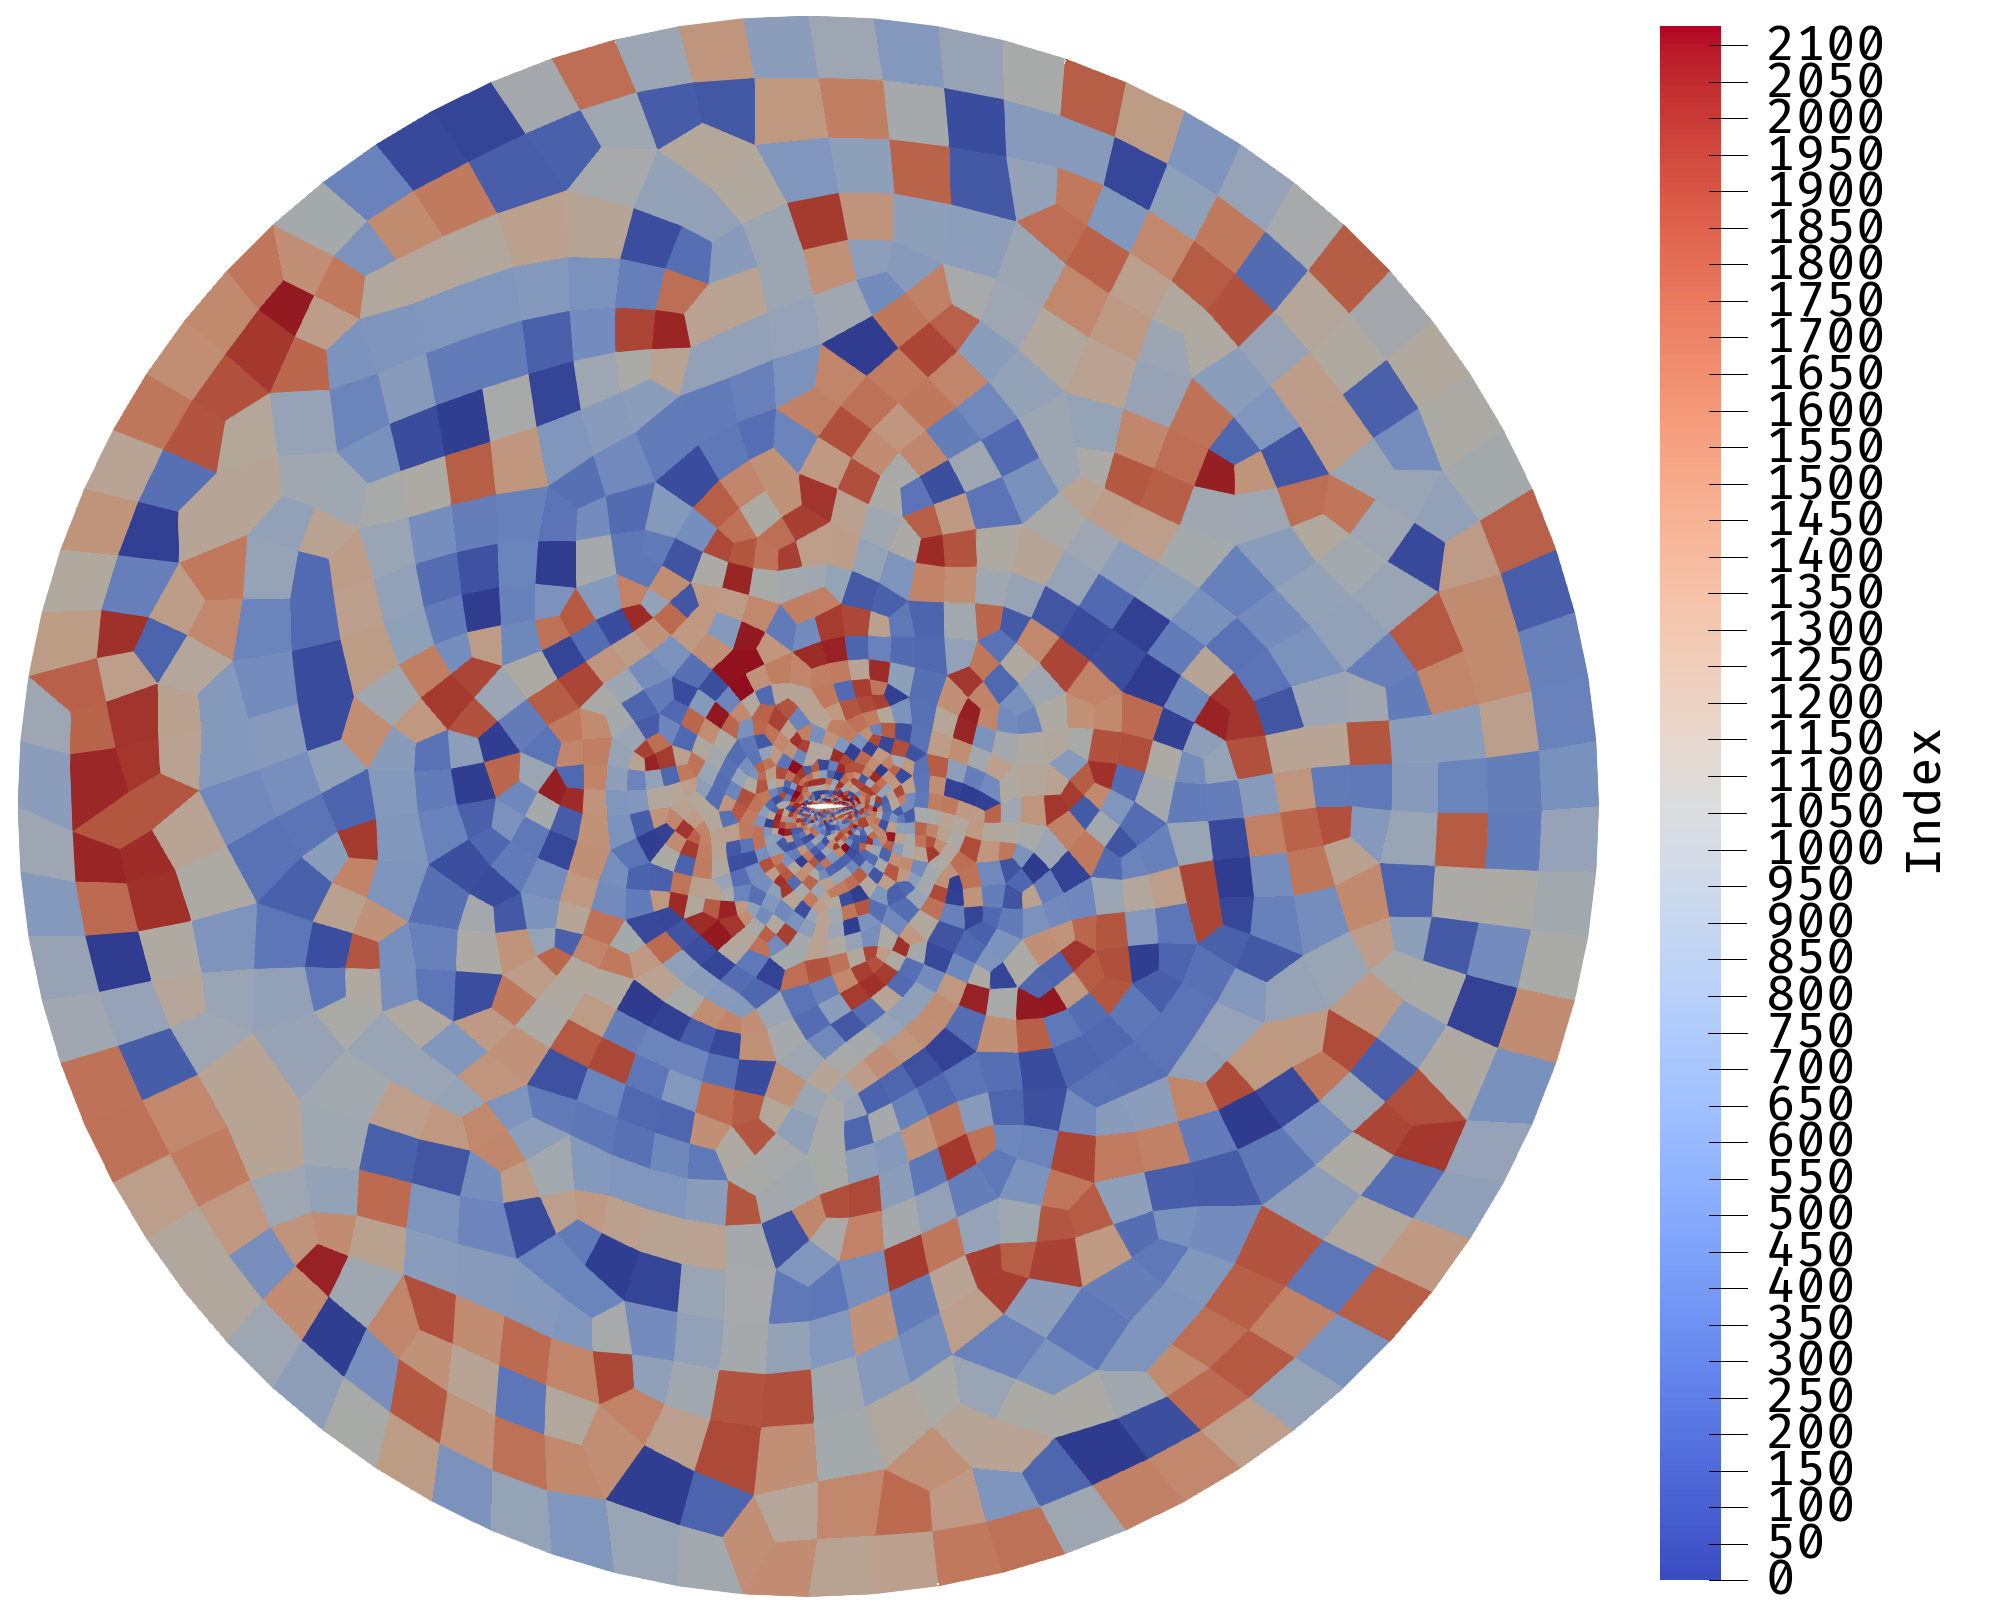
\includegraphics[width=0.45\textwidth]{Chapter_renumbering/media/ordering_unsorted}\label{fig:ordering_unsorted}}
	\subfloat[Rank]
	{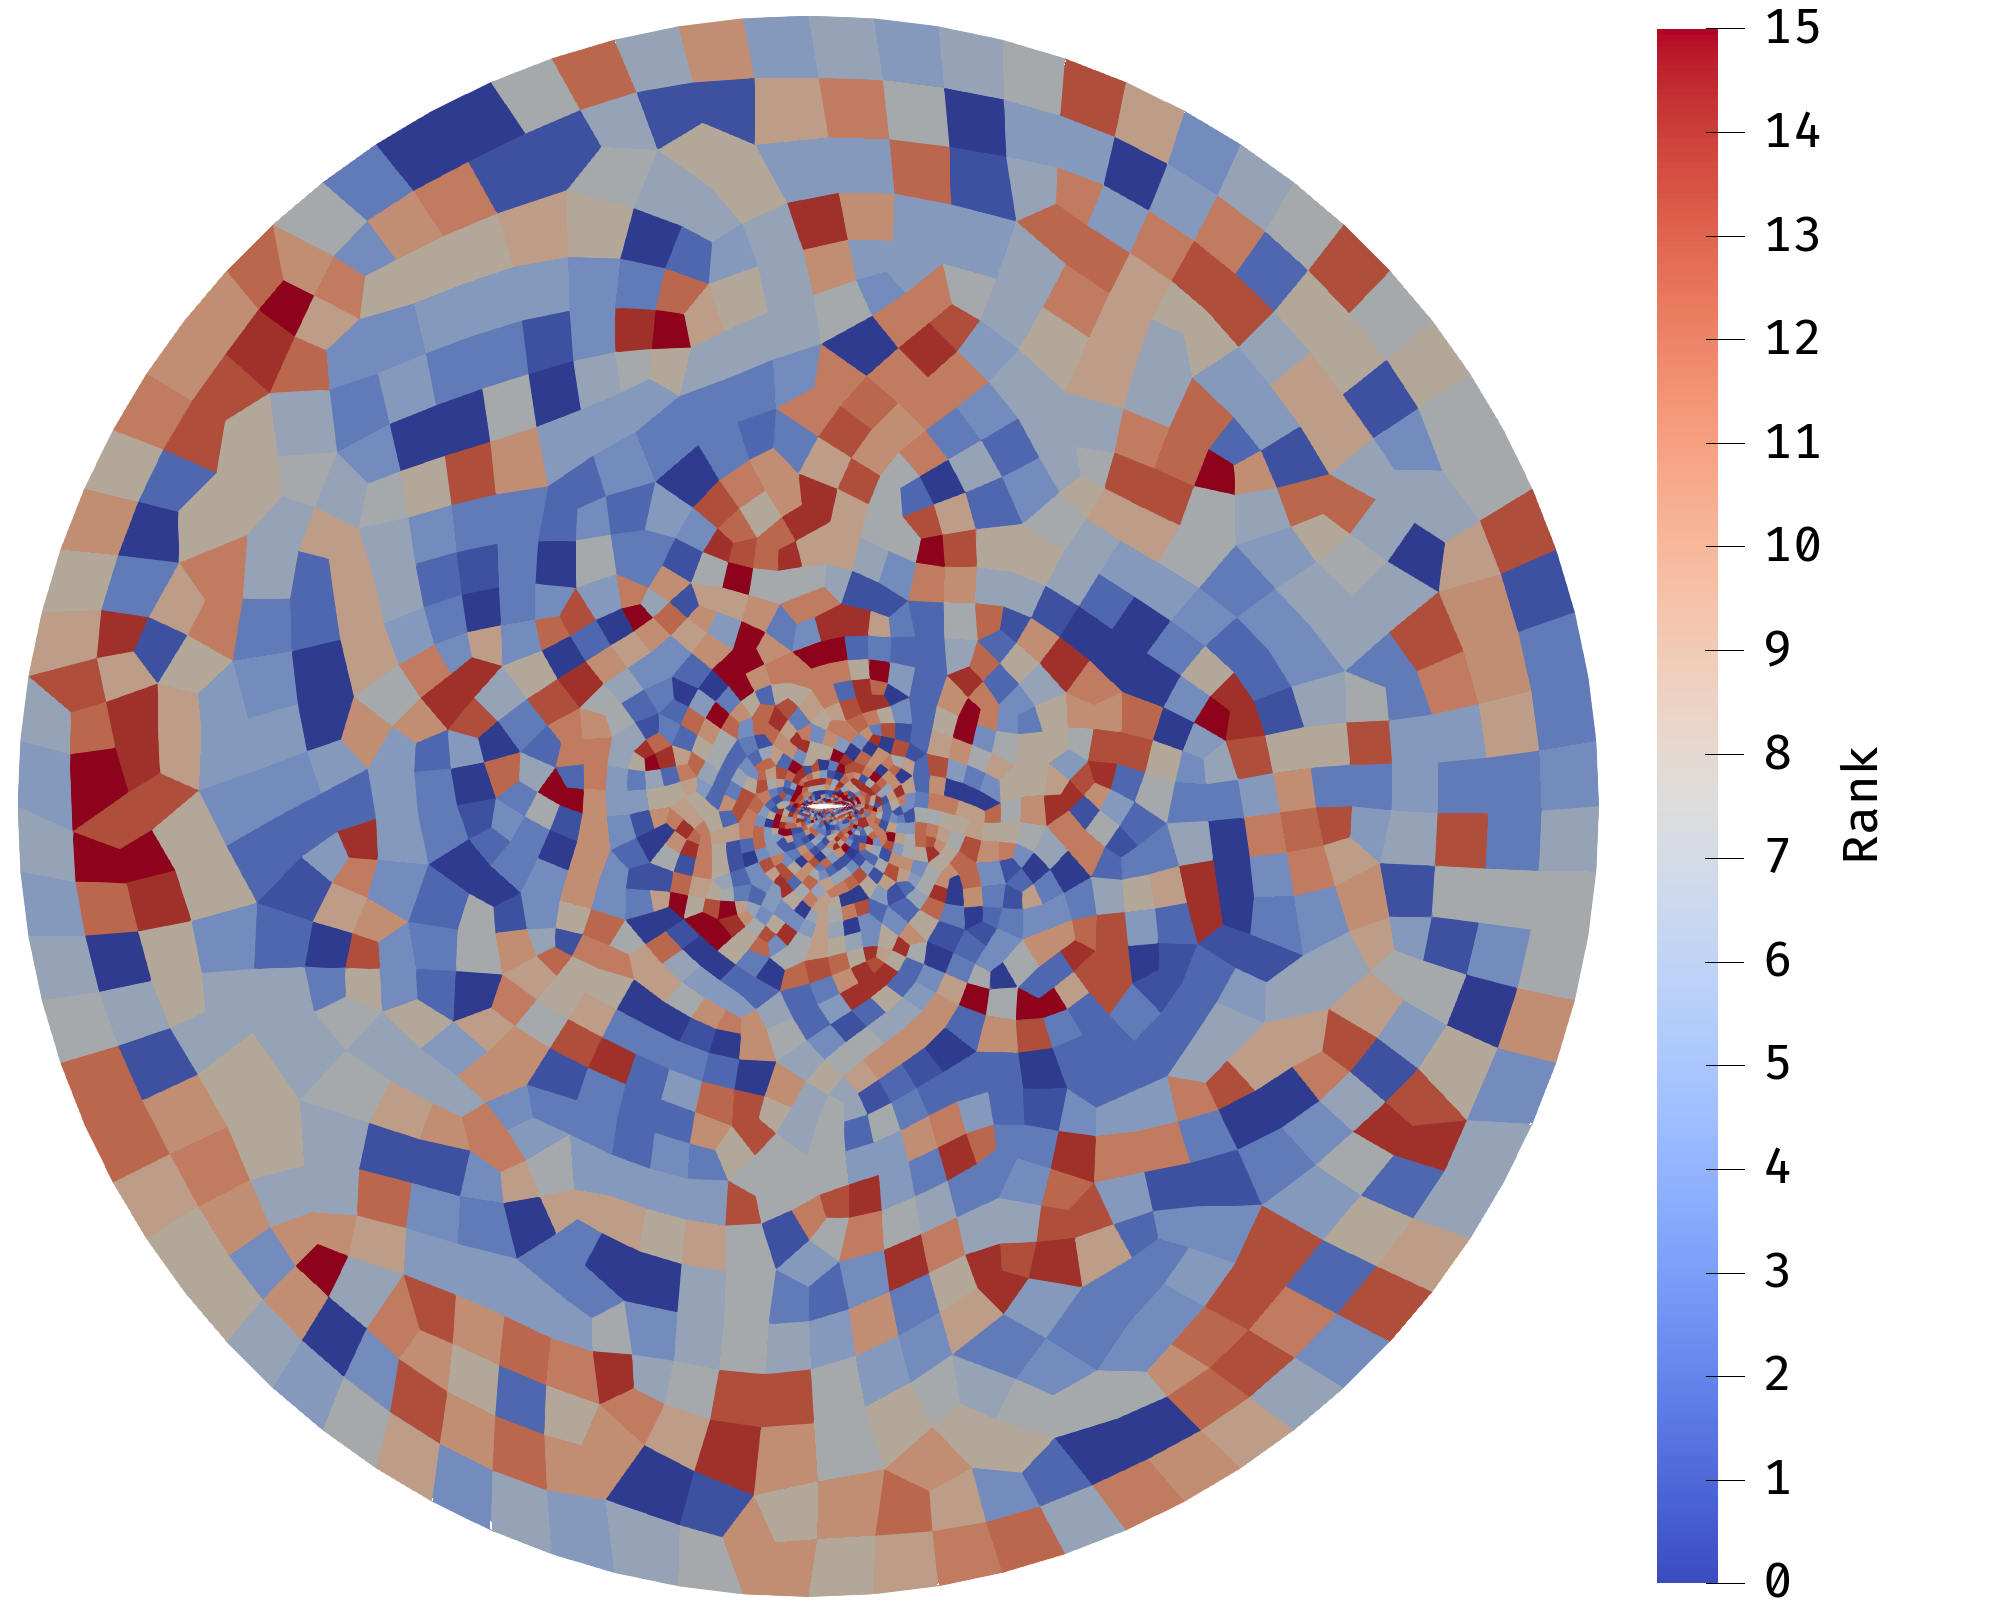
\includegraphics[width=0.45\textwidth]{Chapter_renumbering/media/rank_unsorted}\label{fig:rank_unsorted}}
	\caption{Unsorted mesh: The mesh is partitioned into \(16\) mesh blocks. (a) Ordering of the elements within the mesh (b) Mesh blocks once partitioned}\label{fig:mesh_unsorted}
\end{figure}

The resulting mesh blocks are scattered around the mesh, leading to unnecessarily large boundaries
between blocks. In order to get good performance, we will need to renumber the mesh. 

Since this mesh is circular, and the hole representing the airfoil is in the middle, a simple
sorting algorithm could represent the elements in polar coordinates, and sort them according to
their angle around the center. The resulting ordering and partitioning are shown in
Figure~\ref{fig:mesh_circular}. The index represents how the elements are ordered in the mesh, and
the rank indicates which mesh block they are part of.

\begin{figure}[H]
	\centering
	\subfloat[Ordering]
	{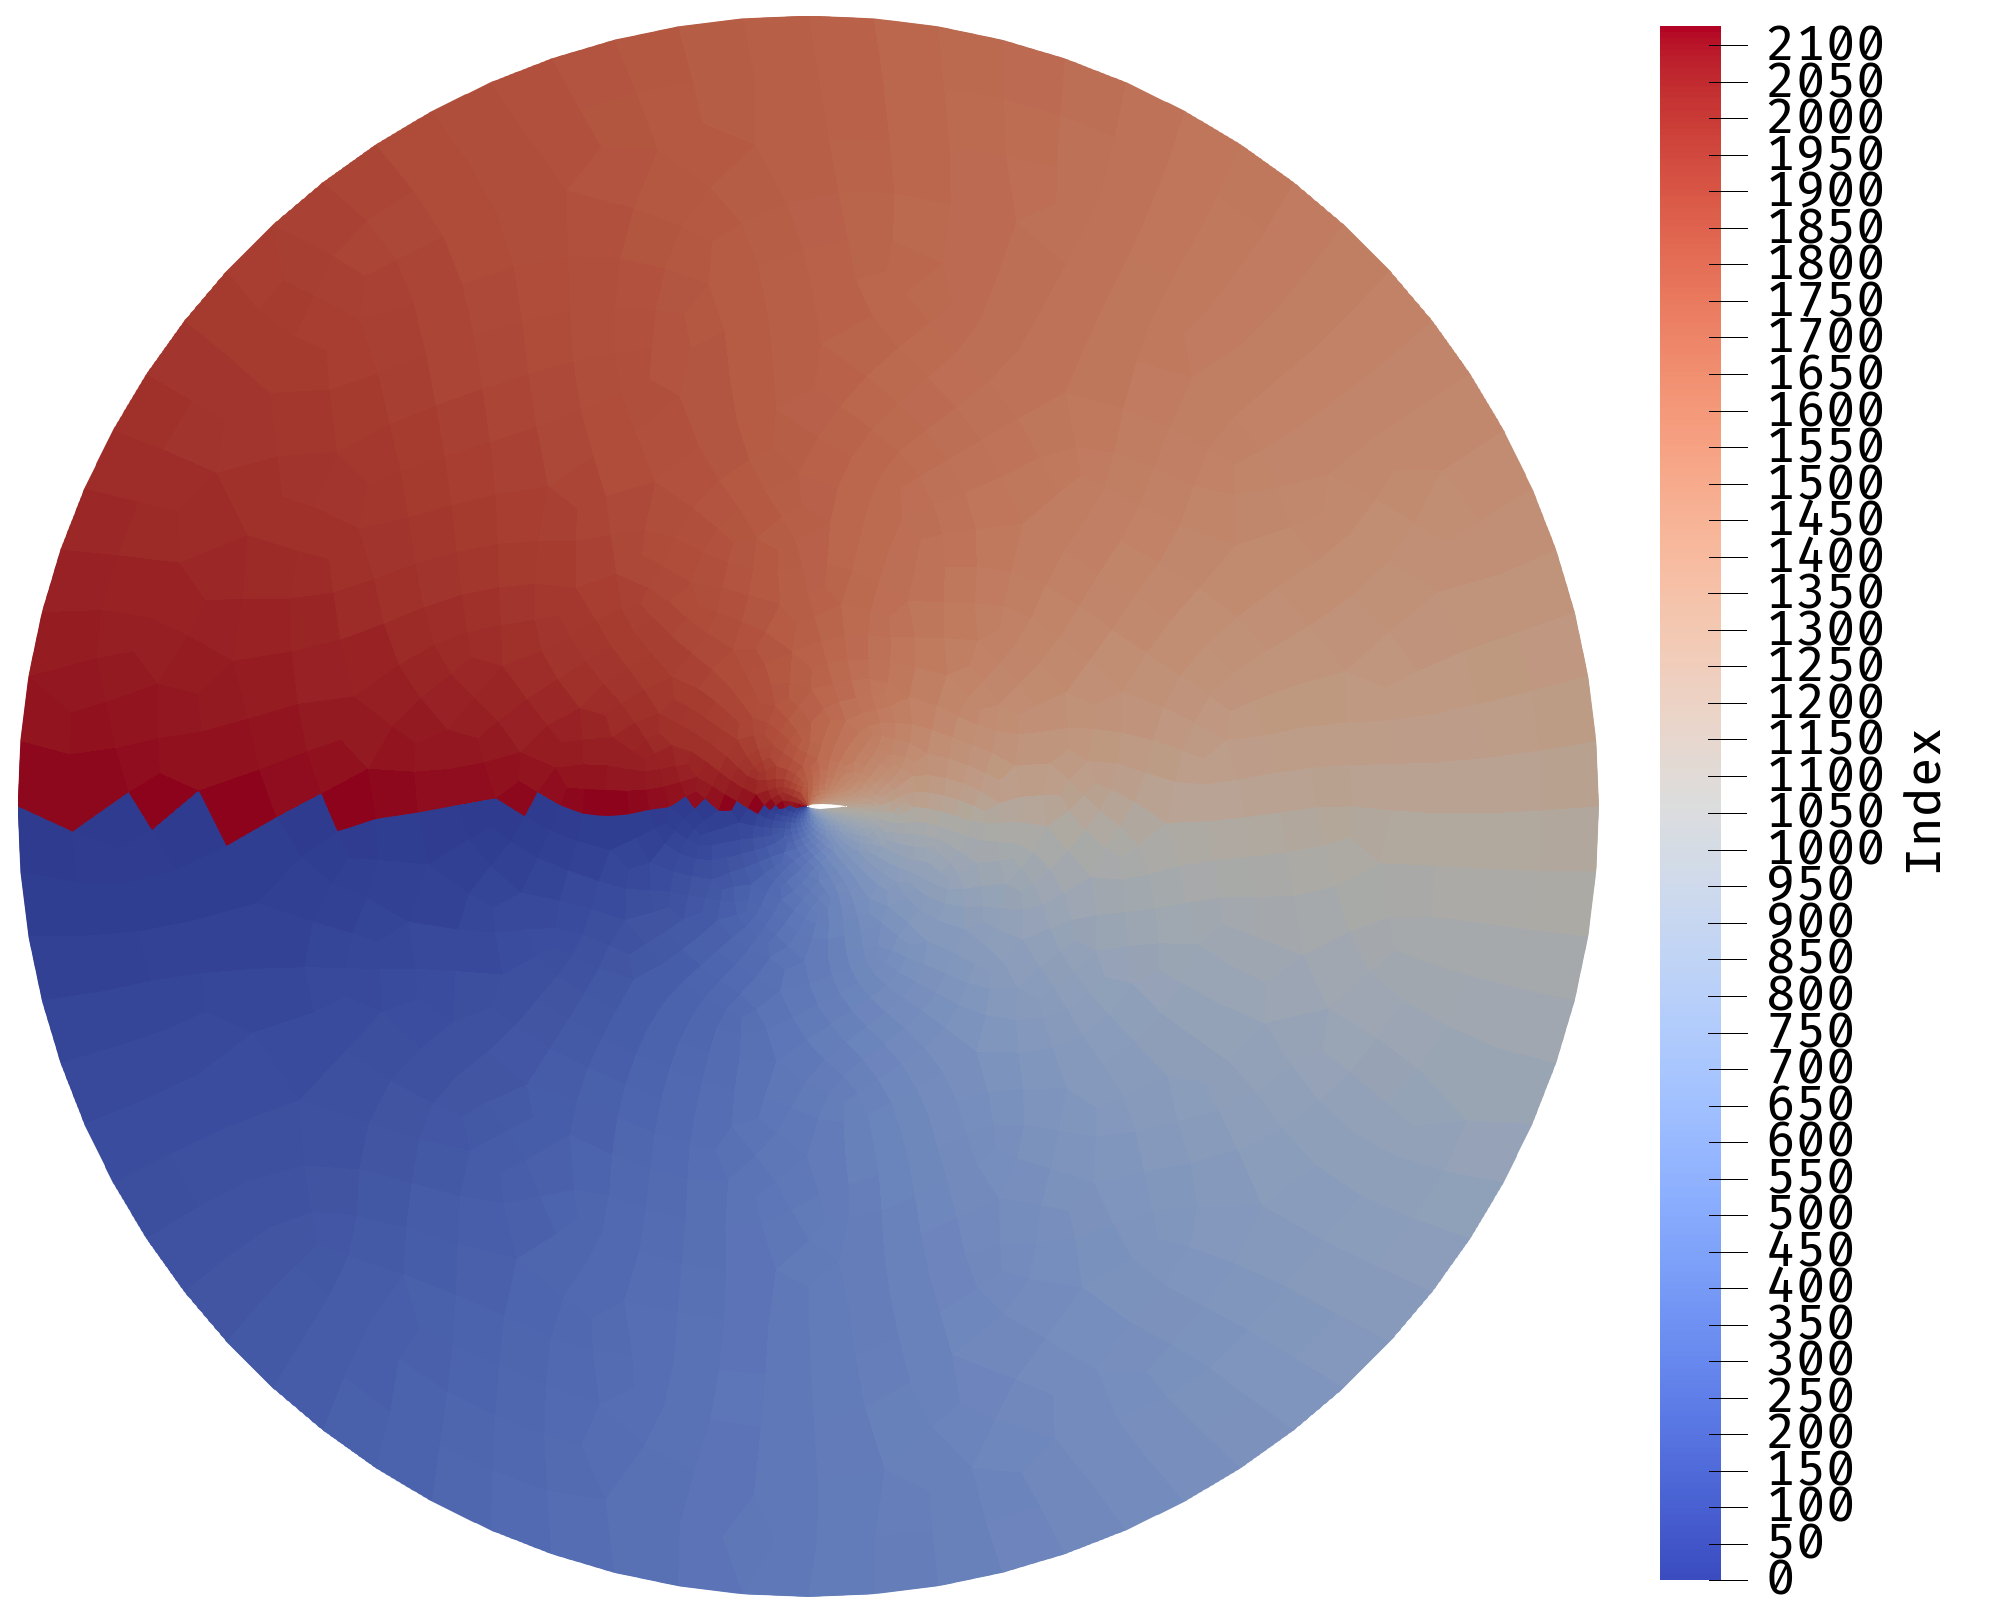
\includegraphics[width=0.45\textwidth]{Chapter_renumbering/media/ordering_circular}\label{fig:ordering_circular}}
	\subfloat[Rank]
	{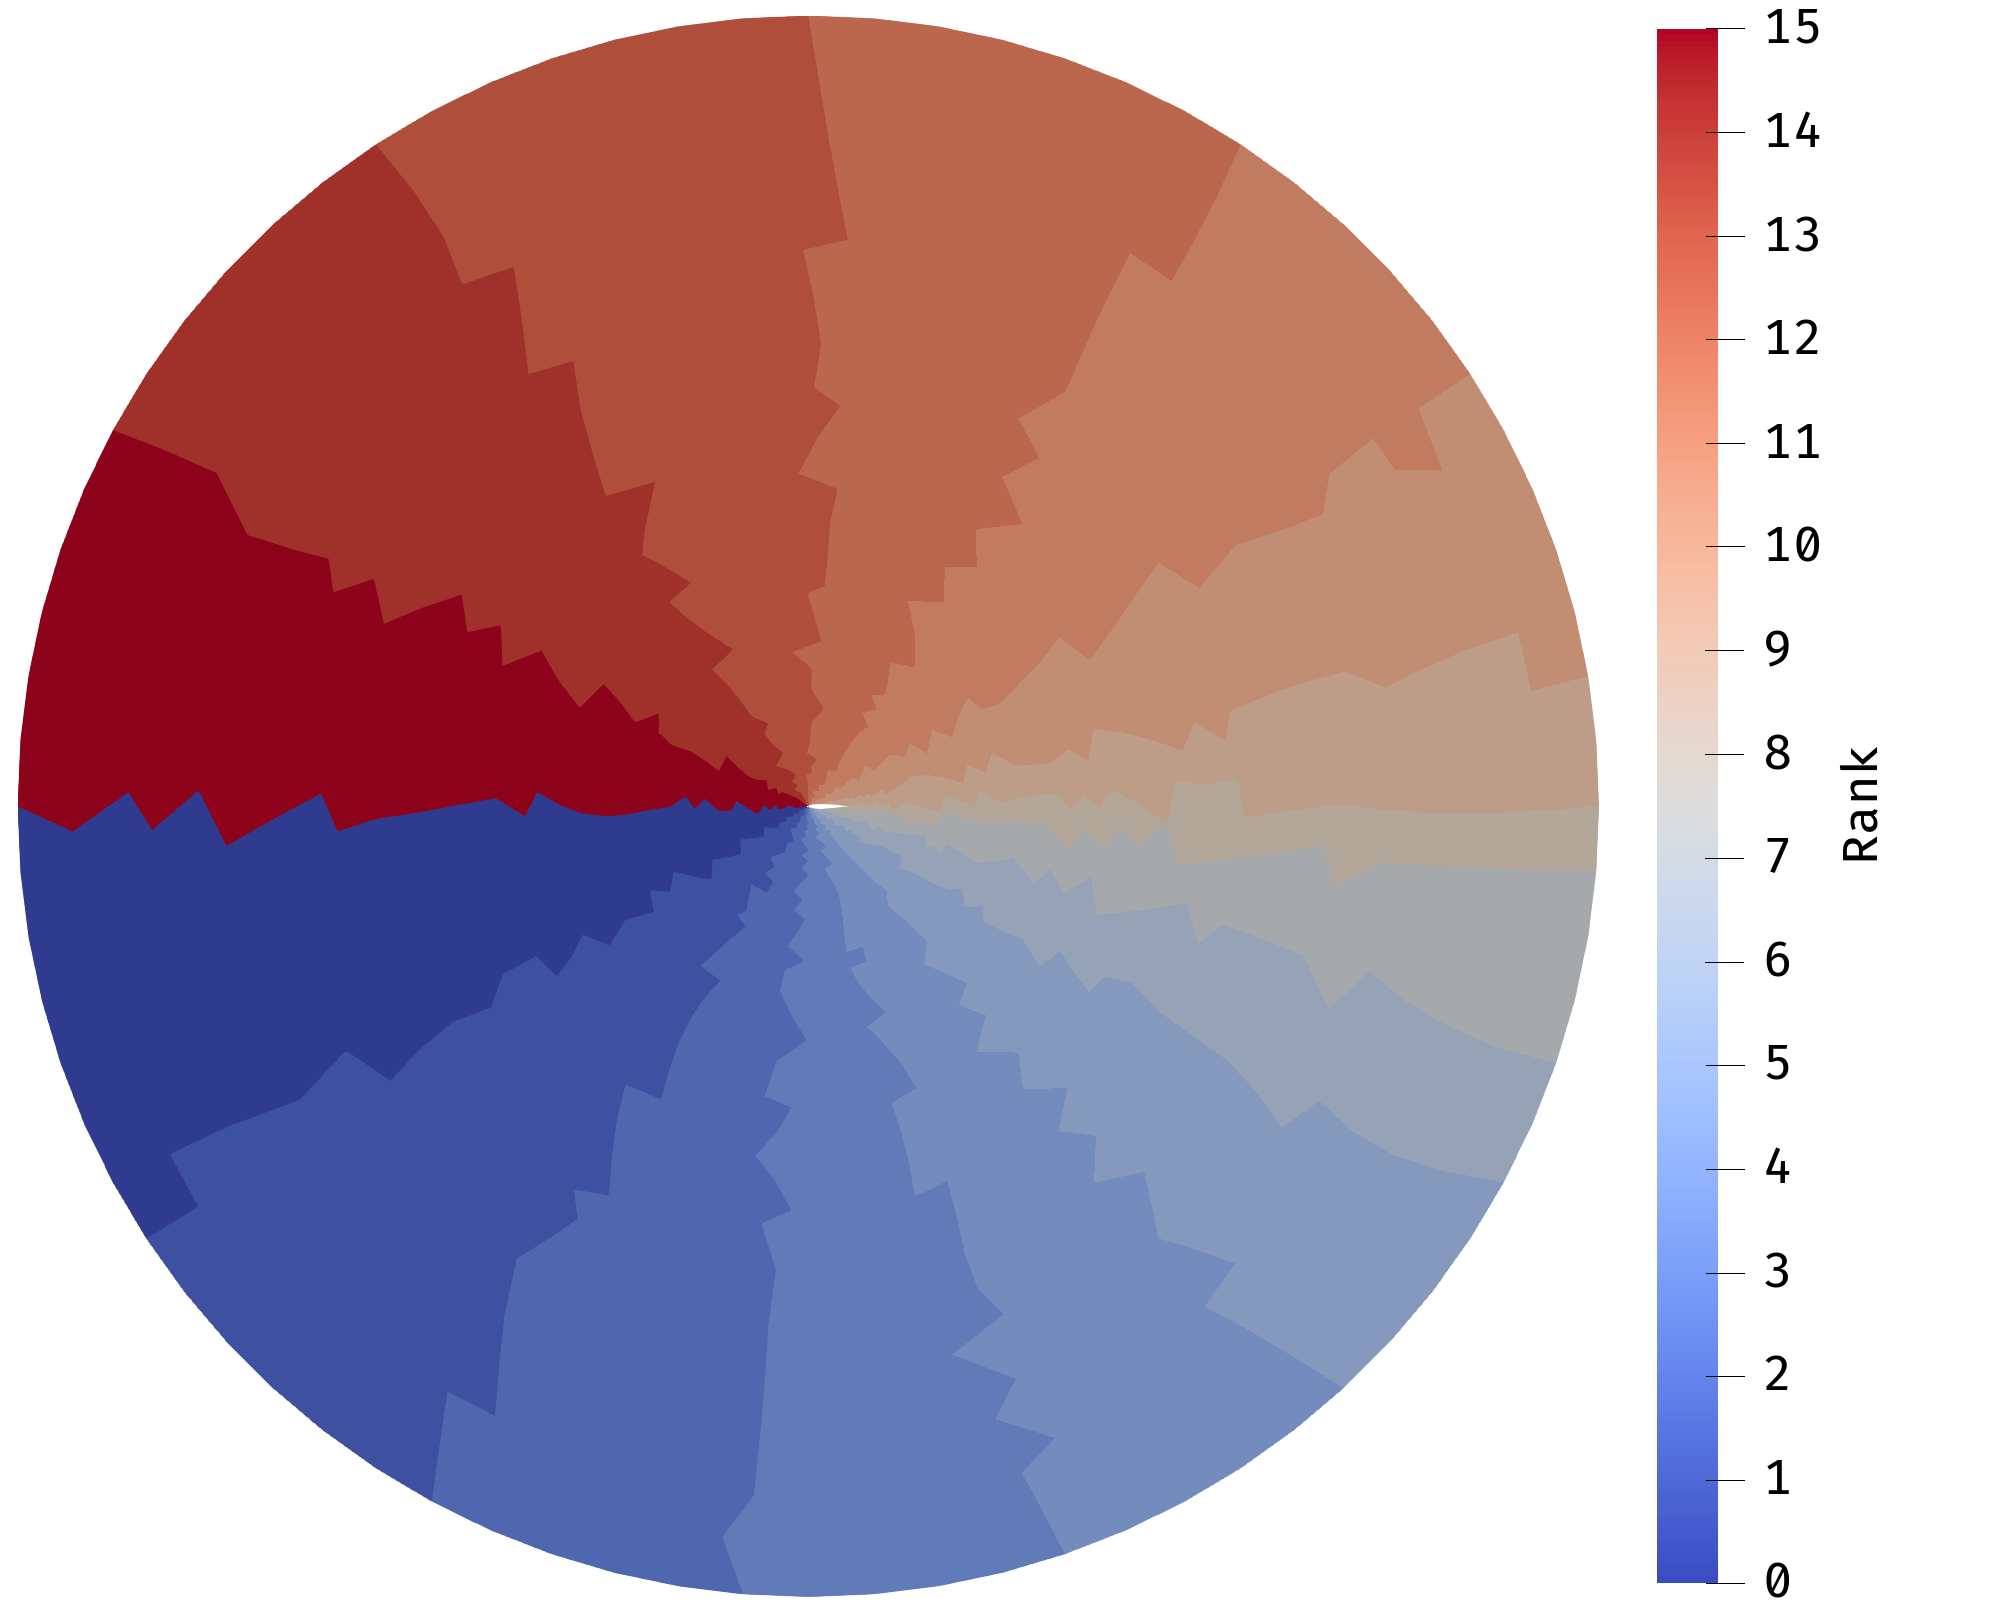
\includegraphics[width=0.45\textwidth]{Chapter_renumbering/media/rank_circular}\label{fig:rank_circular}}
	\caption{Circular sorted mesh: The elements are sorted according to their angle and the mesh is partitioned into \(16\) mesh blocks. (a) Ordering of the elements within the mesh (b) Mesh blocks once partitioned}\label{fig:mesh_circular}
\end{figure}

This method seems to give reasonable results, but is only useful for circular meshes. Also, the
partitions it generates have good grouping for a low number of blocks, but as the number of blocks
increases the blocks become shaped like thin slices. This is not ideal, as it increases the size of
inter-block boundaries. Figure~\ref{fig:mesh_circular_ordering} shows the ordering of elements more
clearly.

\begin{figure}[H]
	\centering
	\includesvg[width=0.98\textwidth]{Chapter_renumbering/media/mesh_P0_before_adaptivity1_circular}
	\caption{Circular sorted mesh element ordering: The elements are very far from their neighbours.}\label{fig:mesh_circular_ordering}
\end{figure}

This is evidently not a good result. Even if this method creates reasonable partitions, the elements
are not necessarily close to their neighbours, which degrades performance.

What we really want is to number the elements according to the Hilbert curve, which gives good
results. As the Hilbert curve is not defined for unstructured geometries like this one, we will have
to approximate it. Firstly we will do an elliptic mapping to transform the circular geometry to a
square. We then generate a Hilbert curve over that square, and number the elements by the 1D index
of where their center falls on the Hilbert curve when rounded to the closest point on the curve. By
sorting the elements by that index, they will be numbered according to the Hilbert curve. If two
elements fall to the same index, they are sorted by their initial index. To avoid this we generate a
very fine, or high level, Hilbert curve. Figure~\ref{fig:hilbert_renumbering} shows the underlying
curve along which the elements are sorted.

\begin{figure}[H]
	\centering
	\includesvg[width=0.98\textwidth]{Chapter_renumbering/media/hilbert_renumbering}
	\caption{Hilbert renumbering: The element centres are rounded to an underlying Hilbert curve.}\label{fig:hilbert_renumbering}
\end{figure}

When we use this method on the same mesh as Figure~\ref{fig:mesh_unsorted}, we obtain a mesh sorted
along a pseudo-Hilbert curve. Figure~\ref{fig:mesh_hilbert} shows the ordering of the elements as
well as the partitions generated.

\begin{figure}[H]
	\centering
	\subfloat[Ordering]
	{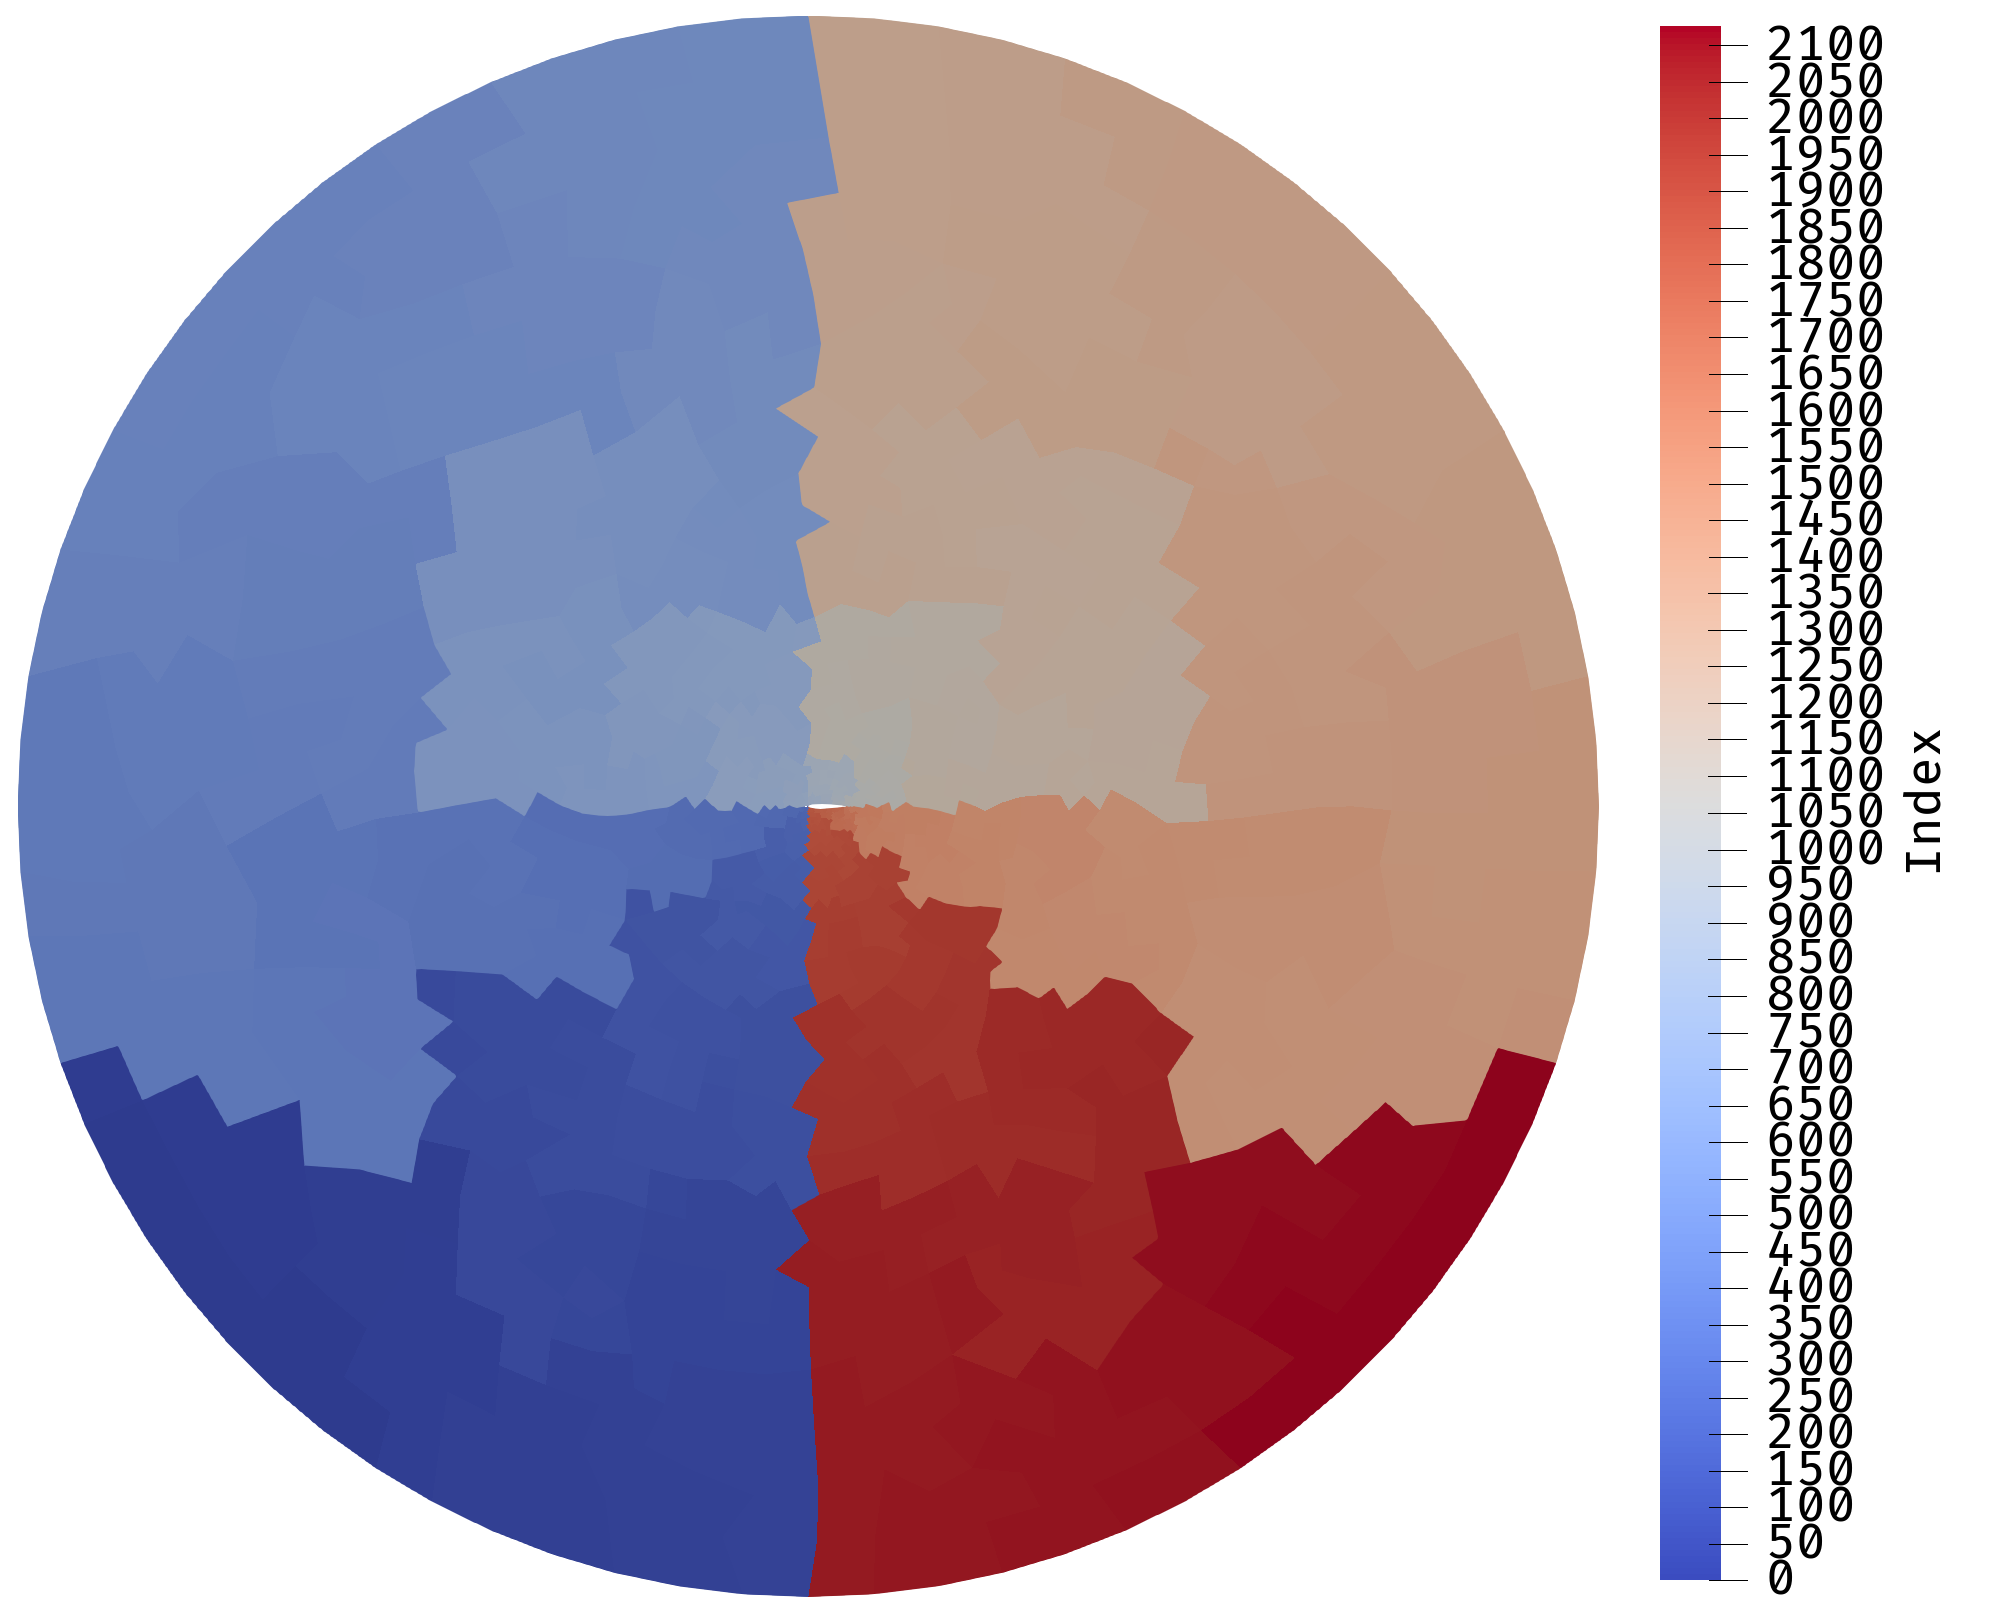
\includegraphics[width=0.45\textwidth]{Chapter_renumbering/media/ordering_hilbert}\label{fig:ordering_hilbert}}
	\subfloat[Rank]
	{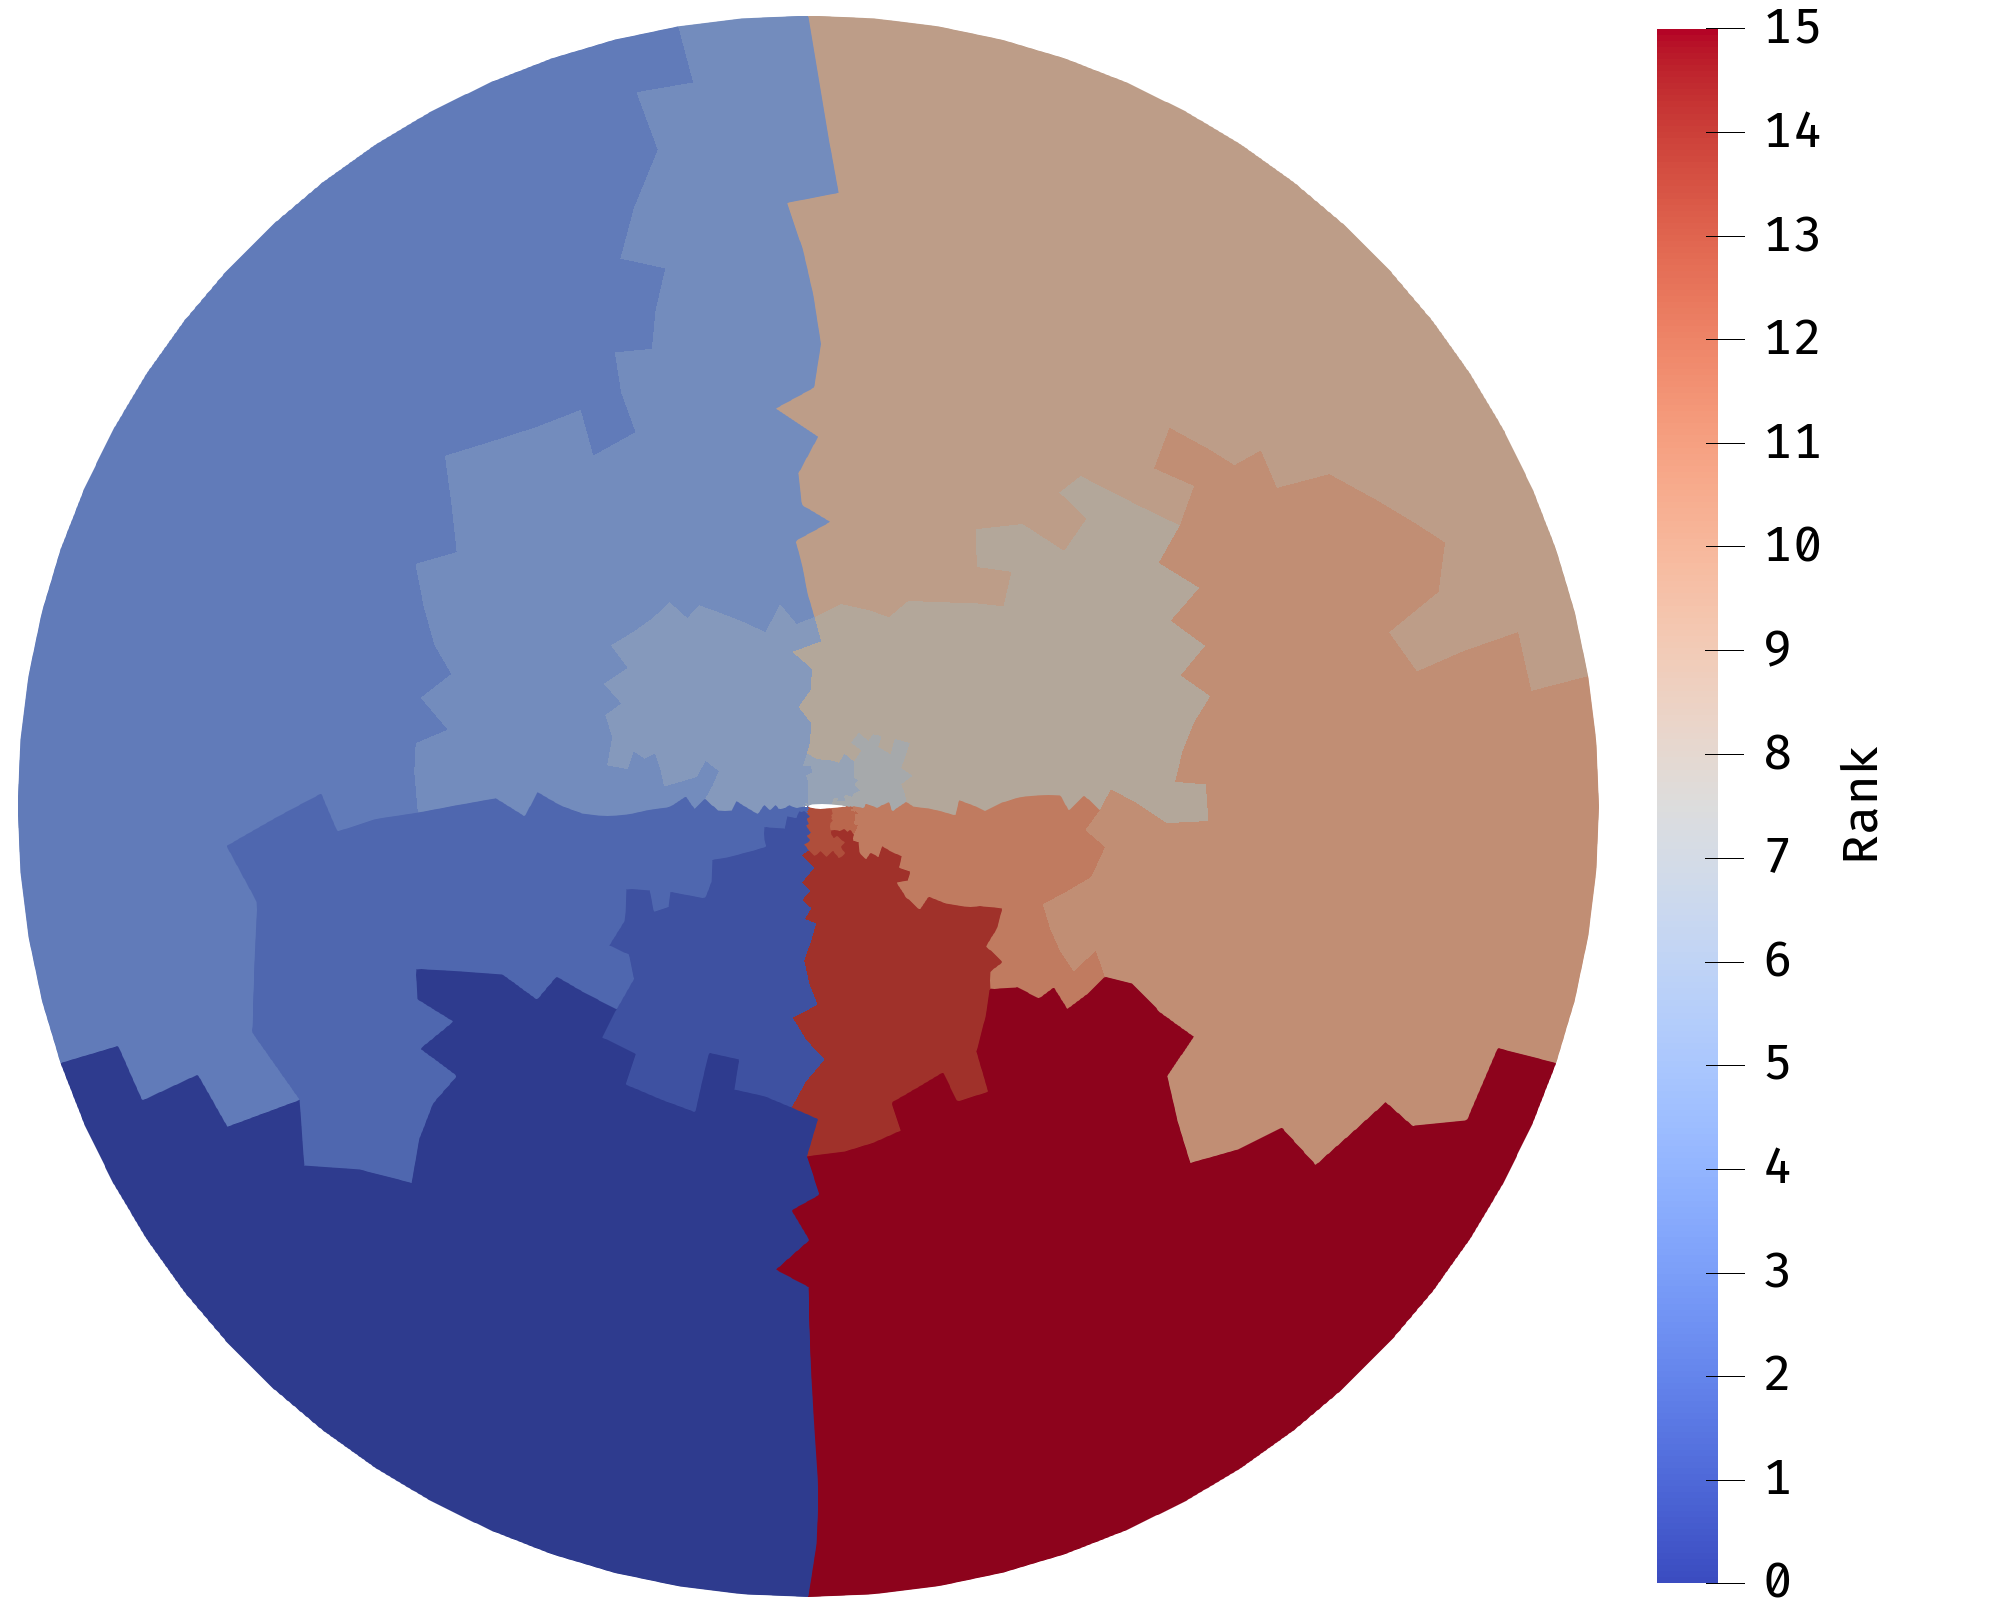
\includegraphics[width=0.45\textwidth]{Chapter_renumbering/media/rank_hilbert}\label{fig:rank_hilbert}}
	\caption{Pseudo-Hilbert sorted mesh: The elements are sorted according to their index along a Hilbert curve, and the mesh is partitioned into \(16\) mesh blocks. (a) Ordering of the elements within the mesh (b) Mesh blocks once partitioned}\label{fig:mesh_hilbert}
\end{figure}

Figure~\ref{fig:ordering_hilbert} shows an ordering that looks a lot like the correct Hilbert curve,
shown in Figure~\ref{fig:correct_hilbert_numbering}. The grouping of mesh blocks in
Figure~\ref{fig:rank_hilbert} is good, and has short inter-block interfaces.


\begin{figure}[H]
	\centering
	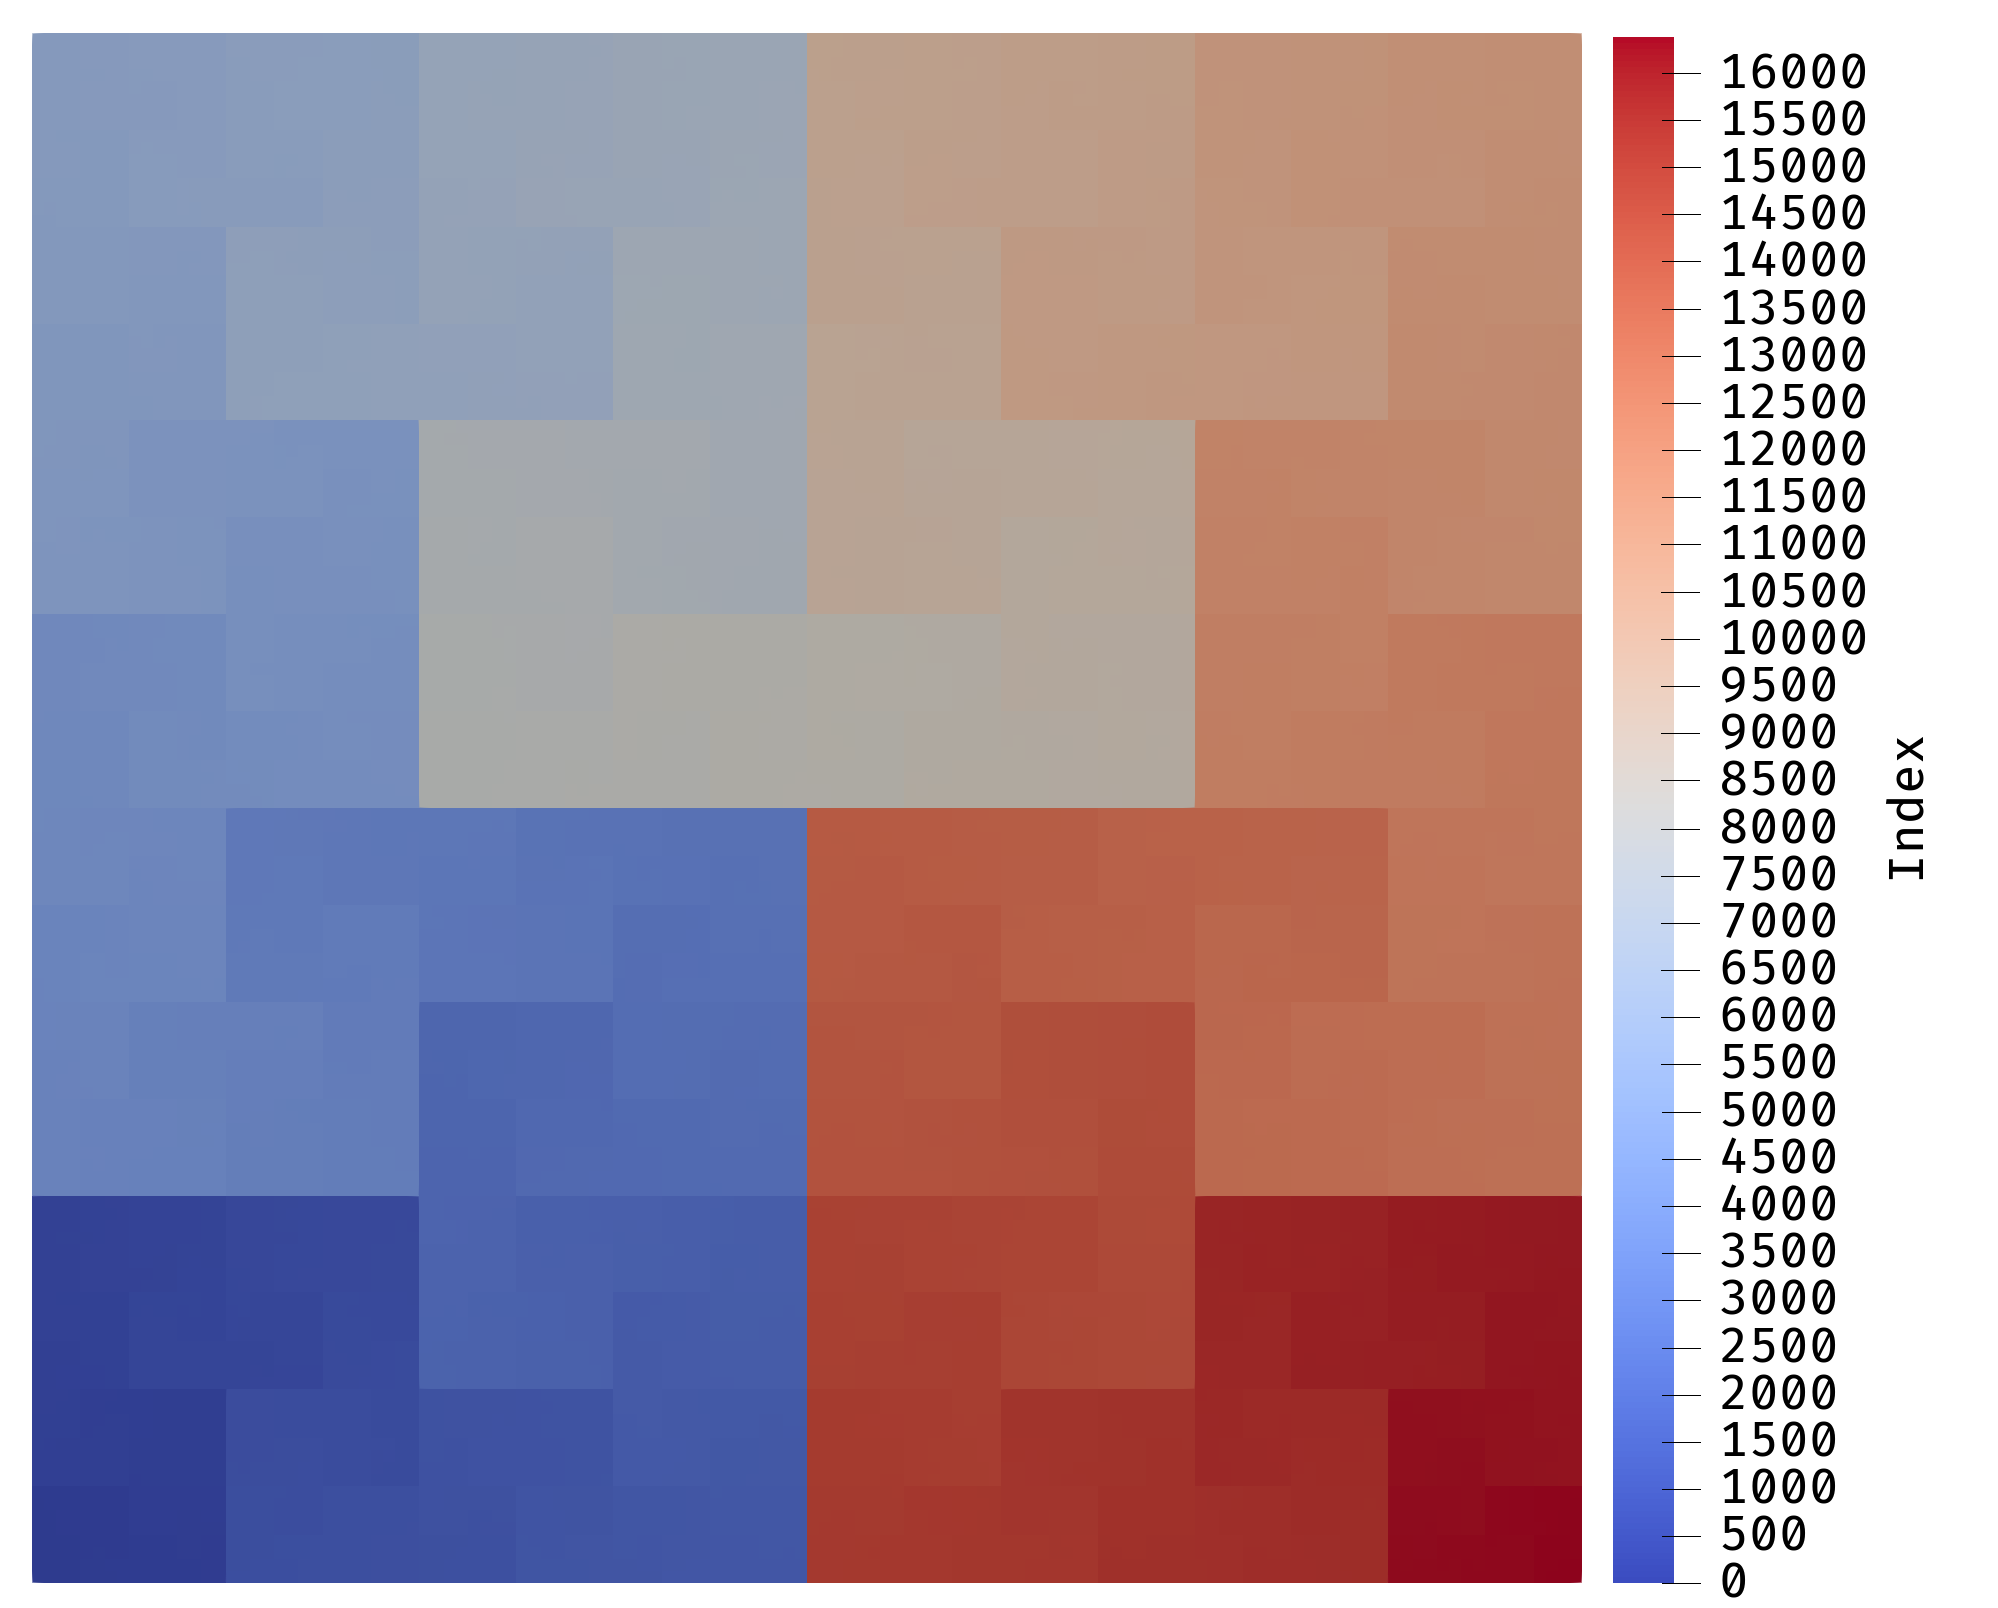
\includegraphics[width=0.45\textwidth]{Chapter_renumbering/media/correct_hilbert_ordering}
	\caption{Correct Hilbert curve: This is the real Hilbert curve, on a \(128 \times 128\) domain where it is defined.}\label{fig:correct_hilbert_numbering}
\end{figure}

Next, Figures~\ref{fig:mesh_P0_adaptivity_far} and~\ref{fig:mesh_P0_adaptivity_near} show the
pseudo-Hilbert curve generated by this ordering method in more detail. We show the mesh before and
after a single refinement step to showcase how the properties of the curve are kept when refining.
Figure~\ref{fig:mesh_P0_adaptivity_far} and~\ref{fig:mesh_P0_adaptivity_near} show the entirety of
the domain and a closer view of the airfoil, respectively.

\begin{figure}[H]
	\centering
	\subfloat[Before refinement]
	{\includesvg[width=0.45\textwidth]{Chapter_renumbering/media/mesh_P0_before_adaptivity1}\label{fig:mesh_P0_before_adaptivity1_far}}
	\subfloat[After refinement]
	{\includesvg[width=0.45\textwidth]{Chapter_renumbering/media/mesh_P0_after_adaptivity1}\label{fig:mesh_P0_after_adaptivity1_far}}
	\caption{\Acrlong{acr:AMR} with an unstructured mesh: The mesh is refined, created elements follow the initial pseudo-Hilbert curve. (a) Initial mesh (b) Mesh after a single refinement step}\label{fig:mesh_P0_adaptivity_far}
\end{figure}

\begin{figure}[H]
	\centering
	\subfloat[Before refinement]
	{\includesvg[width=0.45\textwidth]{Chapter_renumbering/media/mesh_P0_before_adaptivity1_near}\label{fig:mesh_P0_before_adaptivity1_near}}
	\subfloat[After refinement]
	{\includesvg[width=0.45\textwidth]{Chapter_renumbering/media/mesh_P0_after_adaptivity1_near}\label{fig:mesh_P0_after_adaptivity1_near}}
	\caption{\Acrlong{acr:AMR} with an unstructured mesh (detail): The mesh is refined, created elements follow the initial pseudo-Hilbert curve. There are jumps along the curve around the airfoil. (a) Initial mesh (b) Mesh after a single refinement step}\label{fig:mesh_P0_adaptivity_near}
\end{figure}

As the previous figures show, the refinement maintains the path of the curve very well, even if the
initial mesh before refinement shows some problems. Firstly, there are some jumps along the airfoil
and the edges of the domain. This is caused by the fact that the Hilbert curve is not defined for
domains with holes and them. The airfoil is a hole in the domain, and the elements at the edges of
the domain are very big compared to the Hilbert curve resolution, which functionally creates a big
hole on the edge of the domain where there are no elements. Luckily, the Hilbert curve naturally
forms a path around the center of the domain, which is why the pseudo-Hilbert curve also goes around
the airfoil instead of through it. If the airfoil was anywhere else in the domain, the result would
be worse.

Also, the pseudo-Hilbert curve sometimes jumps over elements and sometimes takes surprising paths.
This is because the underlying Hilbert curve along which the elements are sorted is very fine
compared to the elements. The elements are only sorted according to where their centres fall on that
curve, and sometimes the curve will miss the centre of an element and make multiple round trips
before intersecting it, while encountering elements that are further along the way. This can be seen
by looking closely at Figures~\ref{fig:hilbert_renumbering}
and~\ref{fig:mesh_P0_before_adaptivity1_near}, where elements would be sorted very differently if
their centres were moved slightly.

A potential solution to this problem would be to generate a very coarse underlying Hilbert curve,
sorting the elements along that curve, and only refining the parts of the curve where multiple
elements get the same index. These areas would be refined until the elements no longer share
indices. This is future work, as the current incarnation works adequately to show the program
functions well with complex unstructured meshes.

To conclude, this algorithm permits the use of meshes that were not numbered according to the
Hilbert curve, even if the Hilbert curve is not defined for these mesh shapes. The pseudo-Hilbert
curve gives good locality and short inter-block boundaries when partitioning the domain, both
qualities which are crucial to obtaining good performance when using \acrshortpl{acr:GPU}.
